\chapter[Solução Proposta] {Solução Proposta}

A proposta deste projeto envolve a integração dos cinco cursos de engenharia que são lecionados no campus UnB - Gama, com o intuito de resolver os problemas apresentados acima. A proposta inicial de solução se baseia no desenvolvimento de uma biblioteca automatizada, com capacidade de receber um comando do usuário de requerimento do livro, recolher o livro da estante e entregá-lo em cima de uma plataforma, onde o usuário irá poder pegá-lo. Além disso o robô será capaz de fazer o processo contrário, recolher o livro da plataforma e guardá-lo na estante, atualizando o sistema em tempo real.

Este capítulo tem como objetivo apresentar o detalhamento das soluções propostas dos sub-sistemas da \textit{Bibliotech}.

\section{Requisitos do Sistema}
A construção do sistema \textit{Bibliotech} visa atender os seguintes requisitos: 
\begin{figure}[!htb]
     \centering
     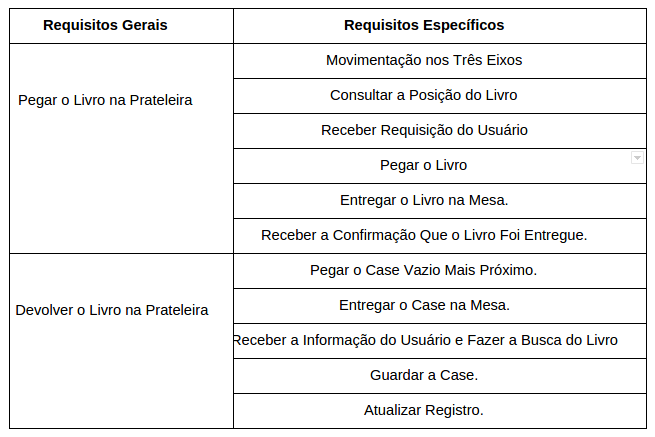
\includegraphics[scale=0.60]{figuras/requisitos}
     \caption{Requisitos do Produto}
     \label{Requisitos do Produto}
\end{figure}
\FloatBarrier

\section[Alimentação]{Alimentação}

O fato do projeto em questão não ser autônomo implica diretamente na escolha da fonte energética do sistema. Tendo isso em mente, o abastecimento será através da rede de energia elétrica local.
Porém, visto que a rede sofre interferências externas resultando em falhas, uma proposta de aconselhável para contornar tal problema é a construção de um sistema de proteção.
Desta forma, o sistema de alimentação será então composto por um quadro de energia, este contendo todos os equipamentos necessários para a proteção dos componentes, um transformador abaixador, tendo em vista que os componentes eletrônicos trabalham com faixa máxima de tensão de 12V e um conversor CA/CC, conforme o fluxograma da figura abaixo: 

\begin{figure}[!h]
\centering
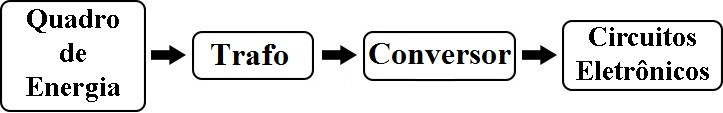
\includegraphics[scale=0.6, angle = 360]{figuras/fluxograma}
\caption[]{fluxograma esquemático da alimentação }
\end{figure}
\FloatBarrier

Os componentes a serem instalados no quadro de proteção são Botão NA, botão NF, Cabo 4mm, Conectores e Fusível.

\subsection{Motor}
A movimentação do robô nos eixos X e Z (considerando Y como profundidade) dependerá de motores, a qual o dimensionamento pode ser encontrado abaixo.

No eixo Z será utilizado um fuso, e a escolha do motor pode ser realizada com base na tabela abaixo:

\begin{figure}[!h]
\centering
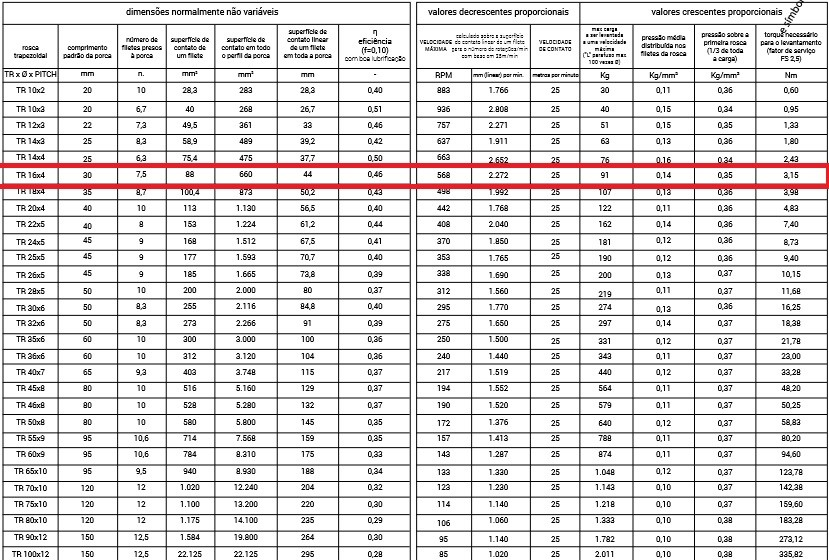
\includegraphics[scale=0.8, angle = 360]{figuras/tabela_escolha_do_motor}
\caption[]{Tabela dos dados do fuso fornecido pela estrutura}
\end{figure}
\FloatBarrier

Já no eixo X, o dimensionamento do motor é feito com base nos seguintes cálculos:

\begin{figure}[!h]
\centering
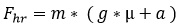
\includegraphics[scale=0.8, angle = 360]{figuras/formula1}
\caption[]{Equação da força horizontal da engrenagem}
\end{figure}
\FloatBarrier

\begin{figure}[!h]
\centering
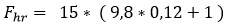
\includegraphics[scale=0.8, angle = 360]{figuras/formula2}
\caption[]{Resolução - Equação da força horizontal da engrenagem}
\end{figure}
\FloatBarrier

O coeficiente de atrito estático foi determinado como sendo 0,12 ,devido ao contato aço – aço. A aceleração da gravidade máxima fixada para o sistema será de 9,8m/s\^2 . A massa total da estrutura da biblioteca será aproximadamente 15Kg

\begin{figure}[!h]
\centering
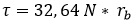
\includegraphics[scale=0.8, angle = 360]{figuras/formula3}
\caption[]{Equação do Torque}
\end{figure}
\FloatBarrier

O raio da base de movimento equivale a 0,1m. Portanto:

\begin{figure}[!h]
\centering
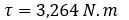
\includegraphics[scale=0.8, angle = 360]{figuras/formula4}
\caption[]{Equação do Torque no eixo do motor}
\end{figure}
\FloatBarrier

A velocidade estipulada pelo escopo da carga é de 0,05 m/s. Sendo assim, têm-se que a rotação do motor dimensionado será de:
 
\begin{figure}[!h]
\centering
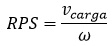
\includegraphics[scale=0.8, angle = 360]{figuras/formula5}
\caption[]{Cálculo da rotação do eixo motor}
\end{figure}
\FloatBarrier

Por fim, RPS=0,08


\begin{figure}[!h]
\centering
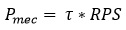
\includegraphics[scale=0.8, angle = 360]{figuras/formula7}
\caption[]{Potencia mecânica total}
\end{figure}
\FloatBarrier

Finalizando, a potência mecânica do sistema é 0.26W

A escolha de um motor com torque aproximado à 
32,64Kgf.cm por valores superiores é aconselhável, desta forma, o motor NEMA 23 com caixa de redução foi escolhido.

\begin{figure}[!h]
\centering
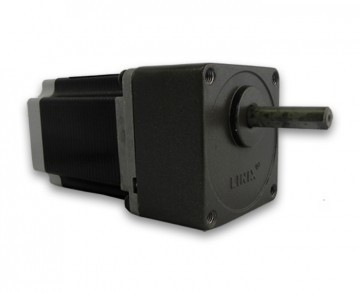
\includegraphics[scale=0.8, angle = 360]{figuras/Motor}
\caption[]{Motor Nema 23}
\end{figure}
\FloatBarrier

\begin{figure}[!h]
\centering
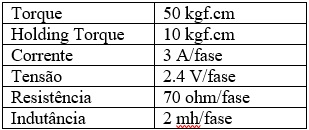
\includegraphics[scale=0.8, angle = 360]{figuras/tabela_unipolar}
\caption[]{Especificações técnicas do motor(unipolar)}
\end{figure}
\FloatBarrier


\section[Estrutura] {Estrutura}
\subsection{Conceito}

O robô será usado em bibliotecas para manipular os livros, assim precisa ser rápido, preciso e durável o suficiente para gerar real benefício. Para isso, será necessário uma estrutura que suporte as forças geradas pelo peso da payload e pela movimentação, sem danos ao robô ou aos livros.

Devido à aplicação e à forma de armazenamento dos livros, serão necessários três movimentos de translação: um paralelo ao comprimento da estante ( Que chamaremos de eixo “x”), um normal ao plano da estante (eixo “y”) e um paralelo à altura da estante (eixo “z”). Para movimentos de translação movidos por motores giratórios, tivemos as seguintes opções:

\begin{itemize}
\item{Correntes, Correias e Cabos}
\end{itemize}

Correntes são muito úteis para a transmissão de várias distâncias, além de muito baratas. Mas por não ser rígida, acaba por não apoiar a movimentação do robô, deixando-o instável. Por conta dessa instabilidade complexa de se tratar, essa opção foi descartada para o uso no projeto.  

\begin{itemize}
\item{Cremalheiras}
\end{itemize}

As cremalheiras são muito usadas em maquinário pesado. São rápidas, com precisão mediana e versáteis: podem ser usadas para movimentos horizontais e verticais. Contudo, movimentos verticais demandam uma estrutura bem mais robusta que aumentaria muito o peso do robô. Sendo assim, essa opção será usada no deslocamento em X, pois nas bibliotecas esse será o maior deslocamento, demandando assim, maior velocidade.

\begin{itemize}
\item{Fusos}
\end{itemize}

Fusos são muito utilizados desde CNC’s a Portões eletrônicos de garagem. São altamente precisos e resistentes, além de possuírem montagem e manutenção simples. Contudo, seu movimento é dependente do passo, o que pode colocar em cheque sua precisão ou o tempo de operação. Como a precisão vertical é a mais permissiva de erros em nosso projeto, optamos por essa solução para o deslocamento em Z, uma vez que o fuso pode ser empregado com um passo grande o suficiente para manter uma velocidade aceitável.

\begin{itemize}
\item{Atuadores Lineares}
\end{itemize}

Atuadores lineares podem ser usados apenas para pequenas distâncias, contudo são extremamente simples e compactos para pequenos movimentos que não requerem precisão. Assim, estes compõem a escolha para movimentos no eixo Y, que simplesmente servirão para trazer o ímã próximo o suficiente do livro para pegá-lo e então de volta para o apoio para o transporte da payload. Devido à pequena amplitude dos movimentos em Y, um atuador linear se torna uma boa opção para esse movimento.

\subsection{Materiais}

Como é um robô de dimensões relativamente grandes - aproximadamente do tamanho de uma pessoa, mas com leves solicitações, é interessante que seja feito com materiais leves e de baixo custo para que o tamanho da estrutura não traga muito mais esforços adicionais nem encarecer o projeto e construção do protótipo.Como cada parte sofre esforços e tem funções distintas, as escolhas de materiais para cada parte será:

\begin{itemize}
\item{Cases}
\end{itemize}

Os compartimentos onde os livros ficam guardados podem ser construídos em madeira, polímero ou metal. No caso de material não-magnético será necessário a aplicação de uma placa de ferro ou aço para que o eletroímã do atuador possa pegar o case com o livro. Visto que não há solicitações estruturais maiores que 2 kgf nos cases, decidimos pelo uso de madeira devido ao baixo peso, custo e facilidade de construção.

\begin{itemize}
\item{Pórtico}
\end{itemize}

O pórtico será feito com barras de alumínio 6063 estrutural de perfil 20x20 devido ao custo de aquisição e facilidade de montagem. O pórtico pode ser montado utilizando parafusos ou soldas, optamos por parafusos devido à praticidade e simplicidade desse método.

\begin{itemize}
\item{Fuso}
\end{itemize}

Fusos podem ser feitos de Alumínio ou aço. Fusos de Alumínio são recomendados para  baixas cargas e velocidades. O fuso será feito de aço porque é o material mais comum dos modelos disponíveis no mercado. A fabricação de um fuso é um processo de difícil execução, portanto a melhor opção é comprar um fuso.

\begin{itemize}
\item{Cremalheira e Engrenagem}
\end{itemize}

Existem duas opções no mercado, cremalheira de aço ou cremalheira de nylon com núcleo de aço. As cremalheiras de nylon são mais indicadas para máquinas leves com velocidades baixas assim como possuem um custo de aquisição menor se comparado às cremalheiras de aço. Por se tratar de uma aplicação leve, usaremos a cremalheira de nylon módulo1.

\subsection{Descrição do produto}

O robô consistirá de um atuador linear, apoiado em uma superfície plana de madeira, que se movimentará na direção vertical por meio de um fuso, e na direção horizontal por meio de uma cremalheira. A estante será subdividida de maneira padronizada, por meio de chapas de madeira, para acomodar cases dentro dos quais estarão os livros. Os cases não só abrigarão os livros como padronizarão o “tamanho” dos livros e suas orientações verticais, para melhor manuseio.

 A movimentação dos livros se dará por um poderoso eletroímã na ponta do atuador linear,que uma vez posicionado, será capaz de aderir-se ao case desejado, puxando-o para a superfície de madeira após o comando retrativo do atuador. Após a retirada do livro para a superfície, o robô se movimentará até uma mesa, posicionada ao lado da estante para a entrega do livro, onde o atuador empurrará o case e desativará seu eletroímã, deixando o livro no local da entrega. Um pórtico de alumínio estrutural garantirá as restrições necessárias para o engastamento do robô ao chão e restrição quanto aos possíveis momentos em torno dos eixos X e Z. A cremalheira será engastada ao chão, enquanto o pórtico também será apoiado em um trilho no topo da estante. Uma solução de baixo custo é o uso de um vergalhão de aço para o trilho.

Abaixo, encontram-se os cads realizados pela equipe de estruturas:
\begin{figure}[!h]		
\centering 
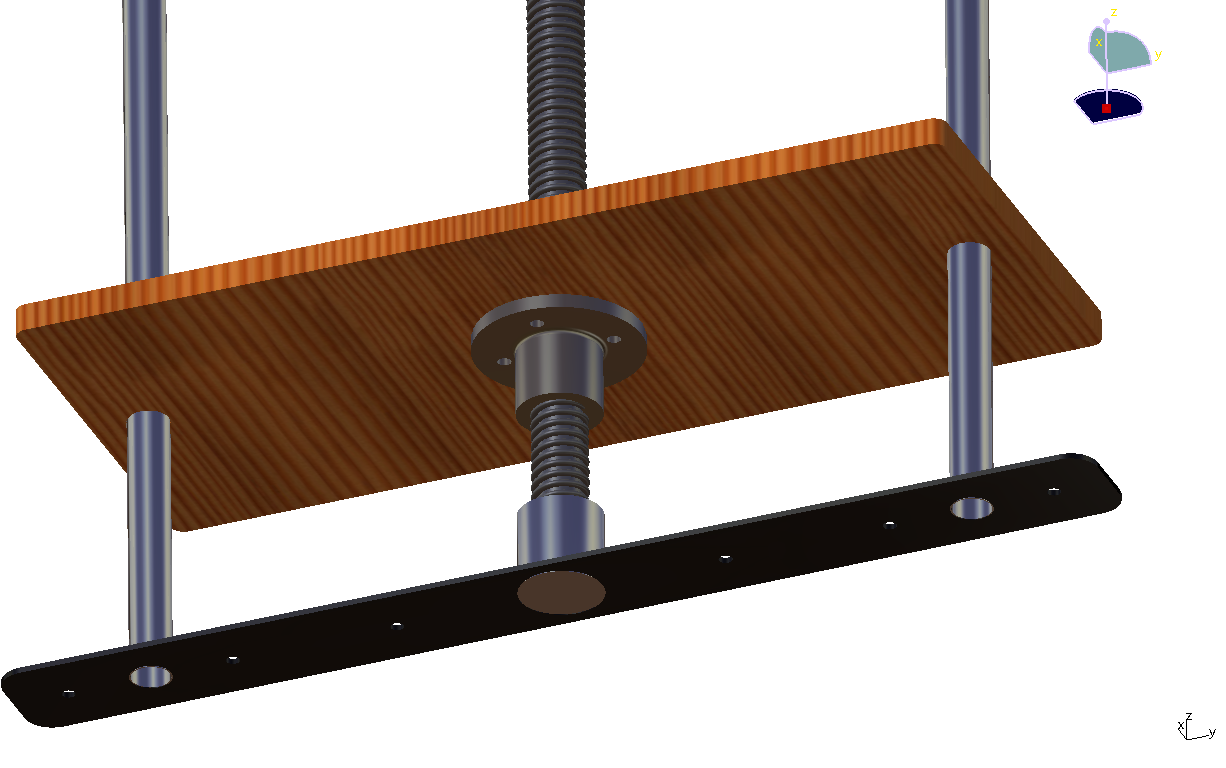
\includegraphics[scale=0.4]{figuras/screen_2}
\caption{Renderização do atuador vertical levemente estendido 40 mm}
\label{Renderização do atuador vertical levemente estendido 40 mm}
\end{figure}
\FloatBarrier

\begin{figure}[!h]		
\centering
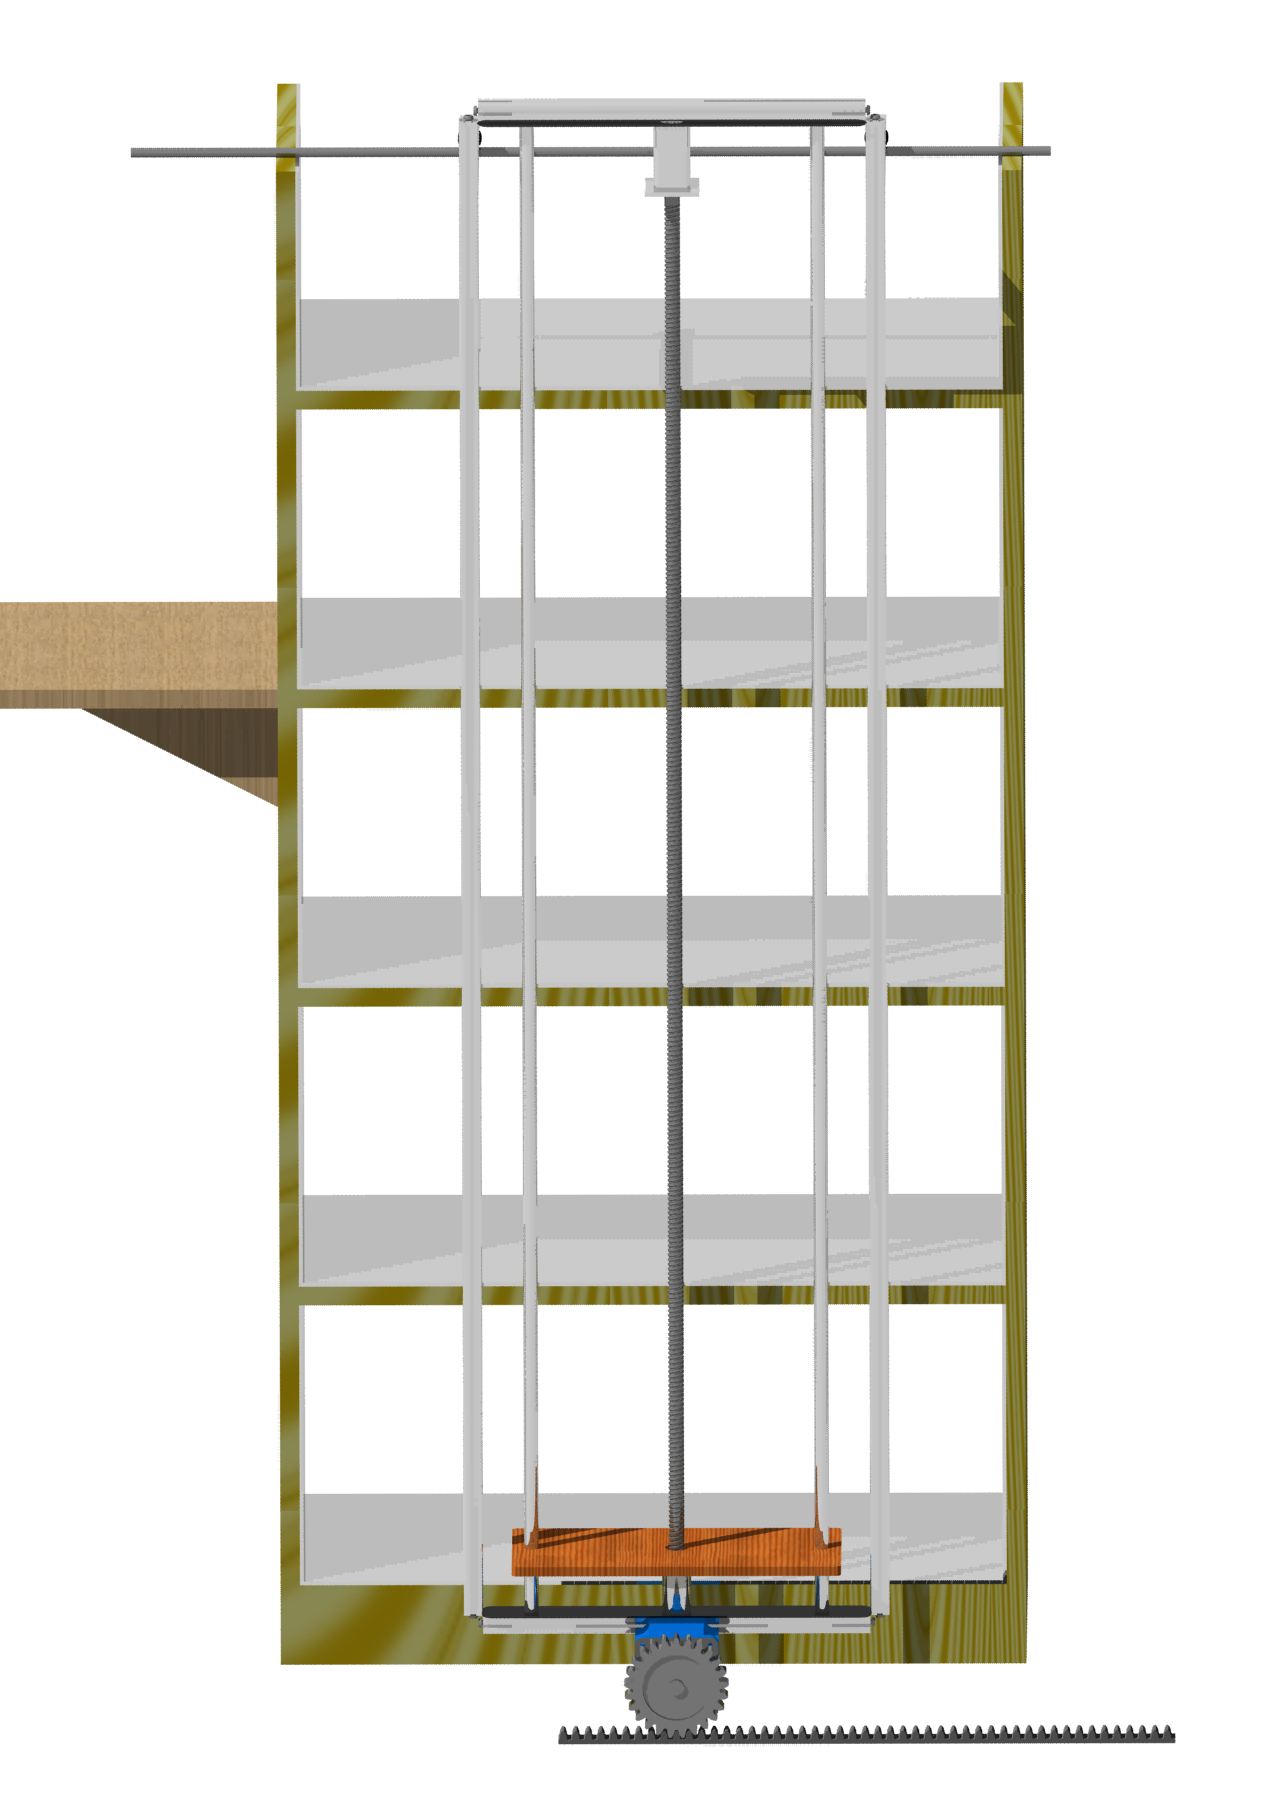
\includegraphics[scale=0.1]{figuras/render_frente}
\caption{Renderização do sistema completo-vista frontal}
\label{Renderização do sistema completo-vista frontal}
\end{figure}
\FloatBarrier


\begin{figure}[!h]		
\centering
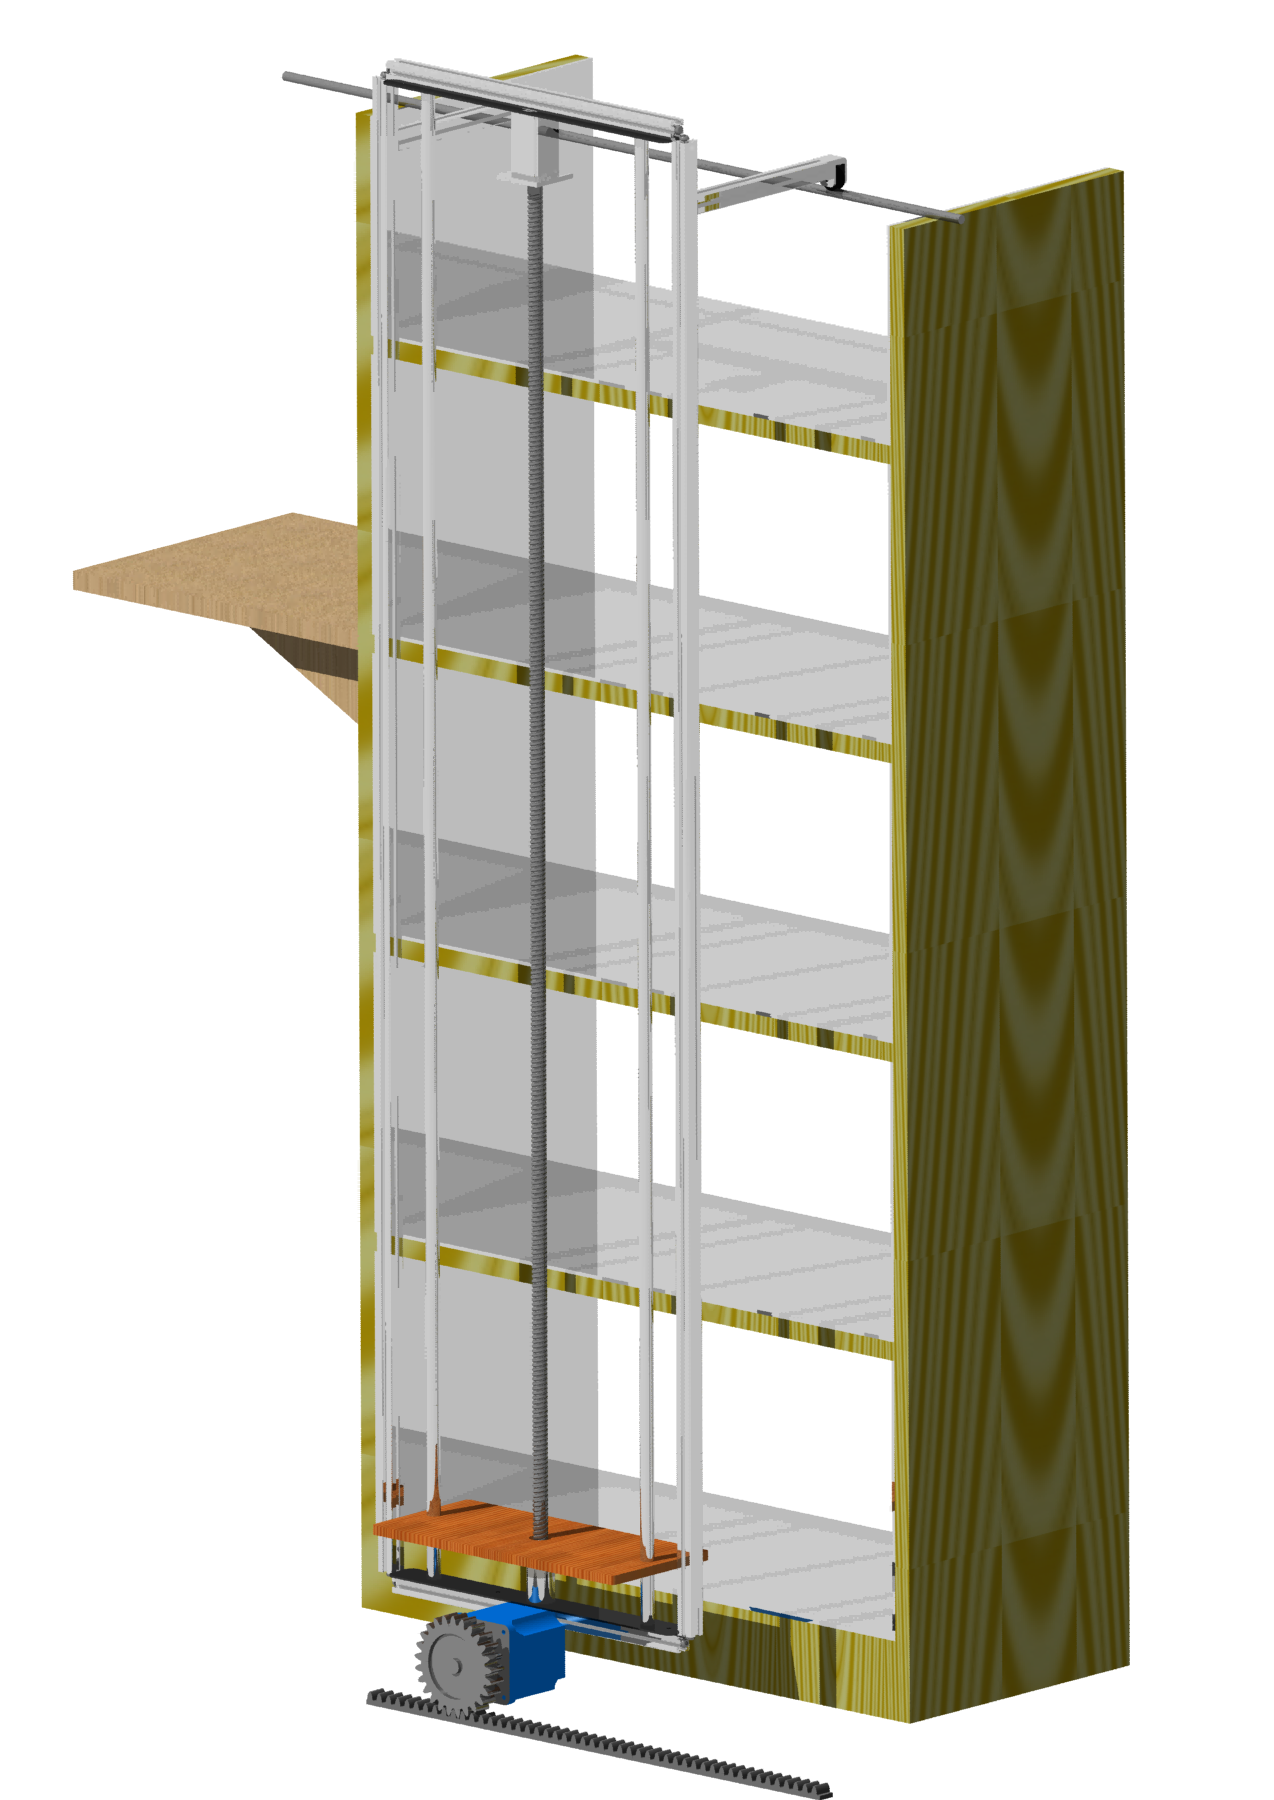
\includegraphics[scale=0.1]{figuras/render_full}
\caption{Renderização do sistema completo}
\label{Renderização do sistema completo}
\end{figure}
\FloatBarrier

\chapter[Sistema Eletrônico] {Sistema Eletrônico}
A parte eletrônica do projeto é dividida em duas categorias: sistema de controle e sistema de comunicação. O sistema de controle é responsável pela movimentação do atuador linear e acionamento do eletroímã. Já a parte de sistema de comunicação, ficará responsável por toda comunicação entre o banco de dados (servidor) e o atuador.

\section{Dispositivo Raspberry PI}
É o principal dispositivo para o funcionamento do sistema de controle e de comunicação, é um computador de baixo custo do tamanho de um cartão de crédito onde tem um poder de processamento bem eficiente para cumprir tudo que o projeto necessita. Este computador, em termos gerais, fará a comunicação entre o pedido do livro, feito pelo usuário, e o funcionamento do atuador para apanhar o livro requisitado na estante. O modelo usado neste trabalho será a Raspberry PI 3. Abaixo é apresentada algumas especificações. (3)

\begin{figure}[!h]
\centering
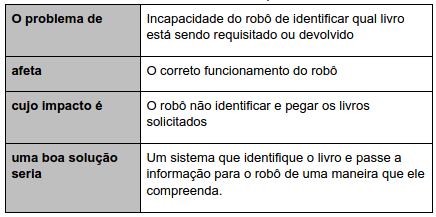
\includegraphics[scale=0.65, angle = 360]{figuras/descricao_problema1}
\caption[]{Problema 01 \footnotemark}
\end{figure}
\FloatBarrier


\begin{itemize}
\item Raspberry Pi 3 Model B.
\item Processador Broadcom BCM2837 64bit ARMv8 Cortex-A53 Quad-Core.
\item Clock 1.2 GHz.
\item Memória RAM: 1GB.
\item Adaptador Wifi 802.11n integrado.
\item Bluetooth 4.1 BLE integrado.
\item Conector de vídeo HDMI.
\item 4 portas USB 2.0.
\item Conector Ethernet.
\item Interface para câmera (CSI).
\item Interface para display (DSI).
\item Slot para cartão microSD.
\item Conector de áudio e vídeo.
\item GPIO de 40 pinos.
\item Dimensões: 85 x 56 x 17mm.
\end{itemize}

\section{Sistema de Controle}
\subsection{Solução 1: Atuador}
Será utilizado um atuador linear (empurra e puxa), fabricado pelos integrantes do grupo (da parte eletrônica), para capturar o livro na estante e levá-lo até o usuário. Na ponta do atuador estará conectado o eletroímã, onde de fato realizará a captura do livro através de sua força eletromagnética. O controle do atuador ficará responsável pela raspberry que terá a incubência de ativa-lo quando chegar no local pretendido. 

\subsection{Solução 2: Braço Robótico}
O braço é a parte da estrutura responsável por agarrar o livro desejado. Como esse sistema irá se movimentar em dois eixos, a padronização dos livros será uma ótima saída. A colocação de cases normalizaria tornando-se mais fácil segurar o livro. O microcontrolador receberia o sinal e apanharia o livro pretendido pelo usuário. Esta estrutura consiste em duas garras que recolheria a case e levaria ao utilizador. Uma enorme parcela da estrutura do braço e do sistema embarcado será executado pela equipe de eletrônica. 

\subsubsection{Movimentação do Braço Robótico}
O funcionamento do braço será composto basicamente por três partes: microcontrolador, servo motor e modulação PWM. O microcontrolador atmega 2650 (comumente chamado de arduíno MEGA)  estará acoplado junto a base do braço robótico, ele irá controlar o movimento mecânico e a captura do livro. O servo motor é o que realizará a movimentação do braço, girando até 180º dependendo do eixo (x,y,z) em que foi colocado. A modulação PWM ditará a posição da movimentação do braço, ou seja, controlará a abertura do braço para posição desejada (ângulo).

Para a captura do livro foi escolhido o eletroímã, assim o microcontrolador terá que cuidar da parte de acionamento do mesmo, onde só será feito depois de comprovado que o livro pretendido de fato está no local estipulado.

\subsubsection{Servo Motor}
São destinados e projetados para uso em aplicações de controle de movimento que exigem posicionamento de alta precisão, reversão rápida e desempenho excepcional.Para manter o controle constante entre o arduino e o servo, é necessário usar um servo motor tipo CC, ele será de baixa potência pois a tensão de alimentação é pequena. Seus componentes são:

\begin{itemize}
\item Motor: Acionamento das engrenagens e eixo principal do servo motor.
\item Engrenagens: Redução de rotação do motor e aumento do torque.
\item Encaixe de saída: conexão de saída do motor.
\item Potenciômetro: Monitora a posição do motor.
\item Circuito de controle: Monitora a saída do potenciômetro e a ativação do motor interno para manter a posição determinada na entrada.
\end{itemize}

\begin{figure}[!h]
\centering
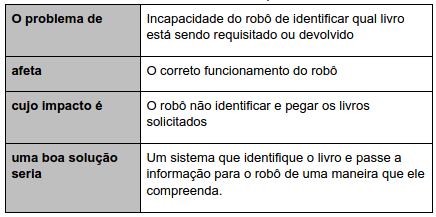
\includegraphics[scale=0.65, angle = 360]{figuras/descricao_problema1}
\caption[]{Problema 01 \footnotemark}
\end{figure}
\FloatBarrier


\subsubsection{Modulçao PWM}

O controle do servo motor é obtido por um sinal de tensão de referência CC, esse sinal é produzido por um gerador de largura de pulso de controle (PWM- Pulse Width Modulation) e servirá para obter a posição angular desejada do motor. Assim com base na figura 1.2 podemos ter a ideia de como funciona. Uma informação é codificada em modulação PWM através da largura do pulso em nível alto em relação ao período total de oscilação, ou seja, através do seu fator de forma (duty cycle).

No PWM tem que ser levado em consideração dois parâmetros, frequência e largura dos pulsos. A frequência é fixa e será gerada pelas saídas digitais do controlador, já a largura varia de tamanho e esse tamanho auxiliará na posição angular do braço.

\begin{figure}[!h]
\centering
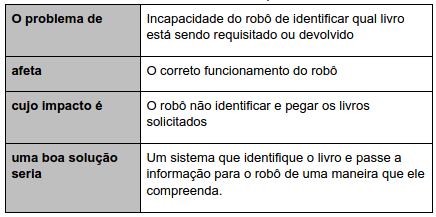
\includegraphics[scale=0.65, angle = 360]{figuras/descricao_problema1}
\caption[]{Problema 01 \footnotemark}
\end{figure}
\FloatBarrier



\subsubsection{Arduino MEGA}
É o microcontrolador que realizará a parte de controle do braço e acionamento do eletroímã. Ele receberá os comandos da raspberry para executar os movimentos para segurar a case contendo o livro requisitado. Suas especificações são:

\begin{figure}[!h]
\centering
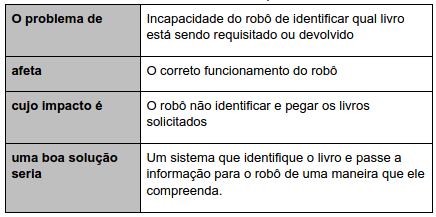
\includegraphics[scale=0.65, angle = 360]{figuras/descricao_problema1}
\caption[]{Problema 01 \footnotemark}
\end{figure}
\FloatBarrier


\begin{itemize}
\item Microcontrolador: ATmega2560.
\item Tensão de Operação: 5V.
\item Tensão de Entrada: 7-12V.
\item Portas Digitais: 54 (15 podem ser usadas como PWM).
\item Portas Analógicas: 16.
\item Corrente Pinos I/O: 40mA.
\item Corrente Pinos 3,3V: 50mA.
\item Memória Flash: 256KB (8KB usado no bootloader).
\item SRAM: 8KB.
\item EEPROM: 4KB.
\item Velocidade do Clock: 16MHz.
\end{itemize}

\subsection{Solução Escolhida}
A solução escolhida será a do atuador, por ser mais fácil a construção, contudo, a solução do braço  não será totalmente descartada a princípio, devido a sua complexidade, pode ser motivada pelo desafio onde aumentará o nível do projeto.

\section{Sistema de Comunicação}
\subsection{Comunicação UART}
A UART (Universal Asynchronous Receiver/Transmitter) como o próprio nome já diz é um sistema de comunicação em que dados digitais são transmitidos e recebidos na forma serial operando no modo assíncrono. Neste projeto, a UART estará presente na comunicação entre a Raspberry e o Arduino, onde o usuário irá escolher o livro através de uma página em uma rede local, a rasp então irá traduzir as escolhas feitas na página em comandos para o Arduino via UART. Para isso é necessário tomar alguns cuidados:

\begin{itemize}
\item BAUD RATE(Clock de operação) : Os dois dispositivos devem possuir o mesmo baud rate, caso contrário não funcionará a comunicação, necessário procurar no datasheet do microcontrolador (na sessão da UART) o cálculo do baud rate. A unidade de operação é em bps (bits por segundo).
\item Configuração do protocolo: O protocolo de UART pode ser configurado para mandar dados de 8 ou 9 bits, com possibilidade de bits de paridade (par, ímpar, nenhum), com 1 ou 2 bits de parada. Os dois dispositivos devem possuir a mesma configuração.
\end{itemize}

\subsection{Leitura do Código de Barras}
A leitura do código de barras será feita manualmente pela bibliotecário onde tem como função informar baixa do livro no servidor quando o usuário pegar o livro e quando chegar novos livros à biblioteca ele adiciona no banco de dados. 


\section{Referência}


\begin{figure}[!h]
\centering
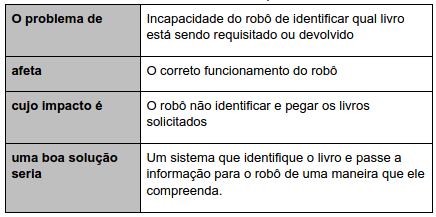
\includegraphics[scale=0.65, angle = 360]{figuras/descricao_problema1}
\caption[]{Problema 01 \footnotemark}
\end{figure}
\FloatBarrier





\section[Sistema Embarcado e Aplicação Web]{Sistema Embarcado e Aplicação Web}

\subsection{Documento de Visão}

Esse documento tem por objetivo fornecer uma visão geral da solução de software a ser empregada para dar suporte às atividades do produto \textit{Bibliotech}. Aqui será descrito o problema a qual o software visa solucionar e dar apoio, o perfil do usuário que estará utilizando o sistema, e uma breve descrição de suas funcionalidades.

\subsubsection{Posicionamento}
Essa seção contém a descrição dos problemas, envolvidos e usuários, e subsequentemente a posição do produto.


\subsubsubsection{Descrição dos Problemas}
Nas figuras abaixo estão descritos os problemas identificados.

\begin{figure}[!h]
\centering
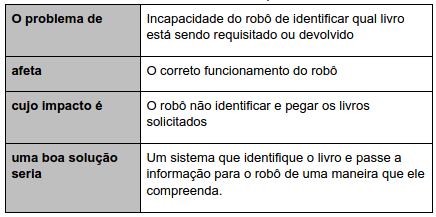
\includegraphics[scale=0.65, angle = 360]{figuras/descricao_problema1}
\caption[]{Problema 01 (fonte: Autor)}
\label{Problema 01}
\end{figure}
\FloatBarrier

\begin{figure}[!h]
\centering
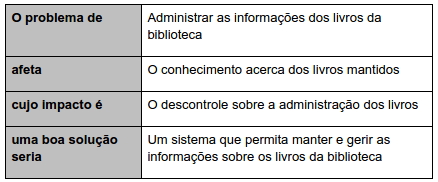
\includegraphics[scale=0.65, angle = 360]{figuras/descricao_problema2}
\caption[]{Problema 02 (fonte: Autor)}
\label{Problema 02}
\end{figure}
\FloatBarrier

\begin{figure}[!h]
\centering
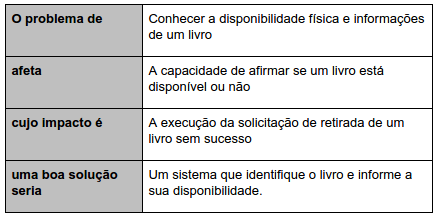
\includegraphics[scale=0.65, angle = 360]{figuras/descricao_problema3}
\caption[]{Problema 03 (fonte: Autor)}
\label{Problema 03}
\end{figure}
\FloatBarrier

\begin{figure}[!h]
\centering
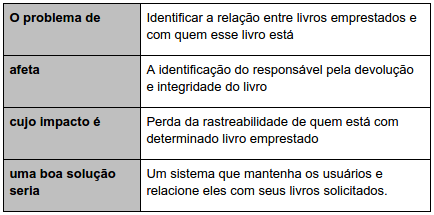
\includegraphics[scale=0.65, angle = 360]{figuras/descricao_problema4}
\caption[]{Problema 04 (fonte: Autor)}
\label{Problema 04}
\end{figure}
\FloatBarrier

\subsubsection{Descrições dos Usuários}
Essa seção apresenta uma descrição geral dos usuários do sistema, assim como suas respectivas responsabilidades e as suas necessidades ao utilizar o sistema.

\subsubsubsection{Resumo dos Usuários}
A a figura abaixo apresenta a descrição de cada usuário do sistema.

\begin{figure}[!h]
\centering
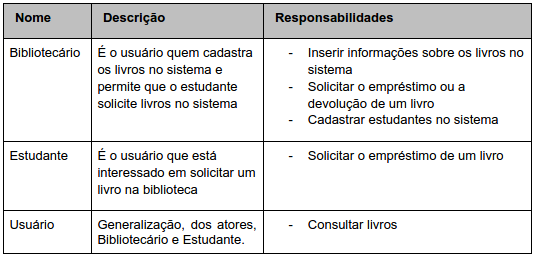
\includegraphics[scale=0.65, angle = 360]{figuras/descricao_usuarios_soft}
\caption[]{Descrição dos usuários do sistema (fonte: Autor)}
\label{Descrição dos usuários do sistema}
\end{figure}
\FloatBarrier

\subsubsubsection{Principais Necessidades dos Usuários}
A figura a seguir apresenta as necessidades dos usuários do sistema, a prioridade e quais são as soluções propostas para cada necessidade.

\begin{figure}[!h]
\centering
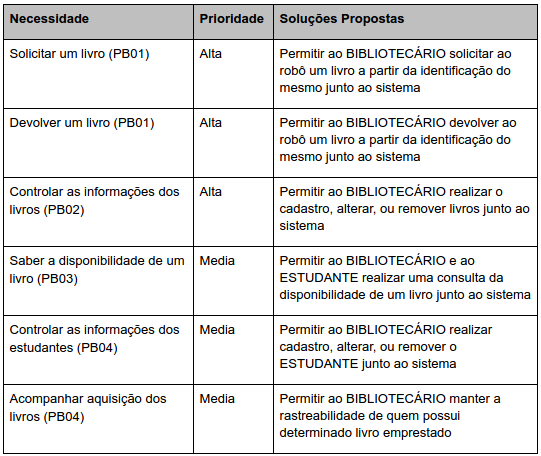
\includegraphics[scale=0.65, angle = 360]{figuras/necessidades_soft}
\caption[]{Necessidades dos usuários do sistema (fonte: Autor)}
\label{Necessidades dos usuários do sistema}
\end{figure}
\FloatBarrier

\subsubsection{Visão Geral do Produto}
Essa seção fornece o detalhamento de como o sistema se relaciona com os outros componentes do produto.

\subsubsubsection{Perspectiva do Produto}
O sistema descrito neste documento faz parte do produto \textit{Bibliotech}. Dessa forma, ele é um subsistema e interage com outros subsistemas, a fim de atingir o objetivo final do produto.

A função do portal é implementar uma interface entre o usuário e o \textit{software} embarcado que realiza o controle das funções do robô. Para isso, ele fornece uma interface \textit{web} que permite ao bibliotecário solicitar que determinadas ações sejam executadas pelo robô. Em última instância, estas solicitações provocam a emissão de uma série de comandos para o robô.

A forma em que o sistema \textit{web} se comunica com o \textit{software} embarcado é através de uma rede \textit{wireless} local. A solicitação da realização de uma tarefa feita pelo usuário gera uma requisição ao \textit{software} embarcado que envia um código específico que indica ao \textit{software} o tipo de tarefa que o robô deve realizar. Desta forma, o \textit{software} embarcado é capaz de determinar quais funções do robô devem ser acionadas.

Após o término da tarefa do robô, o \textit{software} embarcado envia uma resposta ao sistema \textit{web} indicando o status da tarefa. Por fim, o sistema \textit{web} fornece um \textit{feedback} para o usuário indicando o status da tarefa conforme os padrões de usabilidade adotados no projeto.

\chapter[Documento de Arquitetura de Software]{Documento de Arquitetura de \textit{Software}}
Esta seção possui como finalidade apresentar uma visão abrangente da arquitetura dos \textit{softwares} desenvolvidos para o projeto \textit{Bibliotech}. Para isso, serão fornecidas uma série de visões arquiteturais para ilustrar os diversos aspectos do sistema, seus componentes e a forma em que interagem entre si.

\section{Representação Arquitetural}
O projeto \textit{Bibliotech} possui uma série de \textit{softwares} que realizam diferentes funções para garantir o funcionamento do sistema. Cada um destes \textit{softwares} apresenta sua própria arquitetura interna, mas também estão inseridos em uma infra-estrutura externa projetada pela equipe para viabilizar a comunicação entre os subsistemas de \textit{software} . 

Serão descritos os aspectos da infra-estrutura a qual os subsistemas estão inseridos e posteriormente detalhar aspectos relacionados à arquitetura interna de cada um.

Em primeiro lugar, será especificado quais \textit{softwares} compõe o sistema:

\begin{enumerate}
    \item Portal da biblioteca: O portal da biblioteca é uma aplicação web que permite aos bibliotecários gerenciarem os seus livros de forma facilitada. Ou seja, este subsistema implementa a digitalização do empréstimo, adição ao acervo e devolução de livros. O portal abstrai para o usuário todo o processo de gerência de armazenamento implementado logicamente por ele e fisicamente pelo robô. Ele define internamente a administração do uso das prateleiras, por exemplo, quais são as posições livres da prateleira e onde um determinado livro se encontra. Este portal será desenvolvido com o \textit{framework} web Rails.

    \item Sistema Embarcado: Este subsistema é embarcado em uma \textit{Raspberry Pi} e implementa o controle do robô, ou seja, emite uma série comandos que especificam ao robô as operações que devem ser executadas. As principais operações suportadas pelo robô são a movimentação horizontal e vertical (para acessar qualquer parte da estante) e a extração e reposição de um livro a uma posição da estante. Além disso, este subsistema se comunica com o portal da biblioteca para aceitar requisições que especificam a execução de uma função específica (por exemplo, armazenar um livro). Estas requisições disparam a emissão de uma série de comandos internos ao robô para que o mesmo cumpra a função solicitada. O sistema embarcados será desenvolvido em linguagem C.
\end{enumerate}

A figura abaixo fornece uma descrição visual dos \textit{softwares} que compõem o sistema e suas interações.

\begin{figure}[!h]
\centering
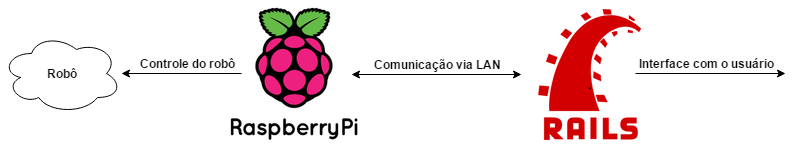
\includegraphics[scale=0.50, angle = 360]{figuras/arquitetura_1}
\caption[]{Arquitetura do sistema (fonte: Autor)}
\end{figure}
\FloatBarrier

O fluxo de execução do sistema pode ser resumido a seguir:

\begin{enumerate}
    \item Portal da biblioteca: O portal da biblioteca é uma aplicação web que permite aos bibliotecários gerenciarem os seus livros de forma facilitada. Ou seja, este subsistema implementa a digitalização do empréstimo, adição ao acervo e devolução de livros. O portal abstrai para o usuário todo o processo de gerência de armazenamento implementado logicamente por ele e fisicamente pelo robô. Ele define internamente a administração do uso das prateleiras, por exemplo, quais são as posições livres da prateleira e onde um determinado livro se encontra. Este portal será desenvolvido com o \textit{framework} web Rails.O bibliotecário interage com a interface web para realizar algum tipo de atividade administrativa (adicionar um livro ao acervo, devolução de livros, empréstimo, etc…). Cada uma dessas atividades administrativas exige um gerenciamento interno do sistema web para identificar o estado das estantes (quais posições estão sendo utilizadas, por exemplo) e dos livros (quais livros estão disponíveis e onde estão armazenados). Para isso, a aplicação web contará com uma base de dados que será responsável por armazenar estas informações. Por fim, o portal da biblioteca enviará requisições ao \textit{software} sendo executado na \textit{Raspberry Pi} informando algum tipo de ação a ser executada.

    \item O servidor sendo executado na \textit{Raspberry Pi} aceitará requisições do portal da biblioteca e mapeará uma requisição a uma série de comandos que especificam ao robô as ações que devem ser tomadas para cumprir a função solicitada.

    \item As funções do robô são acionadas a partir do \textit{software} embarcado na \textit{Raspberry Pi} e após seu término, o servidor envia uma resposta ao portal da biblioteca notificando a conclusão da solicitação enviada.

    \item O portal informa ao usuário que a função solicitada foi executada.
\end{enumerate}

\section{Metas e Restrições da Arquitetura}
Existem algumas metas e restrições arquiteturais consideradas relevantes pela equipe de desenvolvimento, são elas:

\begin{enumerate}
    \item A aplicação web será executada em uma rede local, pois não faz sentido a atribuição de um IP público se ela só será acessada pelos funcionários da biblioteca e se comunicará com o servidor da \textit{Raspberry Pi} que também pertence à rede local.

    \item O portal da biblioteca deve apresentar um sistema de identificação e autenticação que garanta que apenas funcionários autorizados possam acessá-lo com sucesso.

    \item O servidor da \textit{Raspberry Pi} deve aceitar requisições exclusivamente do portal da biblioteca.

    \item A implantação do sistema em uma organização deve ser automatizada, para evitar a configuração manual de IPs para viabilizar a comunicação entre os subsistemas de \textit{software}.
\end{enumerate}

\section{Visão Lógica}
Esta seção se concentra em descrever detalhes arquiteturais internos de cada subsistema:

\begin{enumerate}
    \item Sistema Web: O sistema web será implementado utilizando o estilo arquitetural MVC (\textit{Model}, \textit{View}, \textit{Controller}). Este padrão arquitetural determina a subdivisão do \textit{software} em camadas com responsabilidades específicas:

    \subitem Model: responsável por representar as entidades envolvidas no projeto e implementar a interface entre o sistema e a base de dados.

    \subitem View: responsável por conter o código relacionada à camada visual da aplicação.

    \subitem Controller: responsável por coordenar o fluxo de execução do sistema e atuar como a interface entre as camadas descritas anteriormente.
    
    A aplicação web também será responsável por administrar o uso das estantes. Para isso, o projeto implementa um recurso de discretização das estantes. A discretização é possibilitada pela construção de cases de tamanho único que irão envolver os livros, dessa forma, o espaço ocupado por cada livro é determinístico e o \textit{software} é capaz de interpretar a estante como uma matriz binária, onde cada posição da estante pode ser representada por um par ordenado. Este par ordenado será armazenado para identificar a posição exata de um determinado livro.


    \item Sistema Embarcado: O sistema embarcado será dividido em dois módulos principais:

    \subitem Servidor: responsável por aceitar requisições do sistema web e processá-las para identificar quais comandos devem ser enviados para o robô, além de enviar mensagens de resposta informando ao portal o estado da execução da tarefa solicitada.

    \subitem Controlador: responsável por enviar comandos para o robô para acionar suas funções. Cada função do robô está associada a um dispositivo externo, por exemplo, um motor de passo. Estes dispositivos são representados internamente por um arquivo de dispositivo. A comunicação entre o \textit{software} e os dispositivos periféricos será realizada através destes arquivos e da interface de programação unificada fornecida por sistemas Unix-like para manipulação de arquivos.
    
\end{enumerate}




\subsection[Modelo de Caso de Uso]{Modelo de Caso de Uso}
Este documento apresenta o modelo de caso de uso, onde é desenvolvido um esquema e modelo básico das funções pretendidas do sistema e respectivamente os atuadores em seu ambiente. 

\subsubsection{Diagrama de Caso de Uso}
\begin{figure}[!h]
\centering
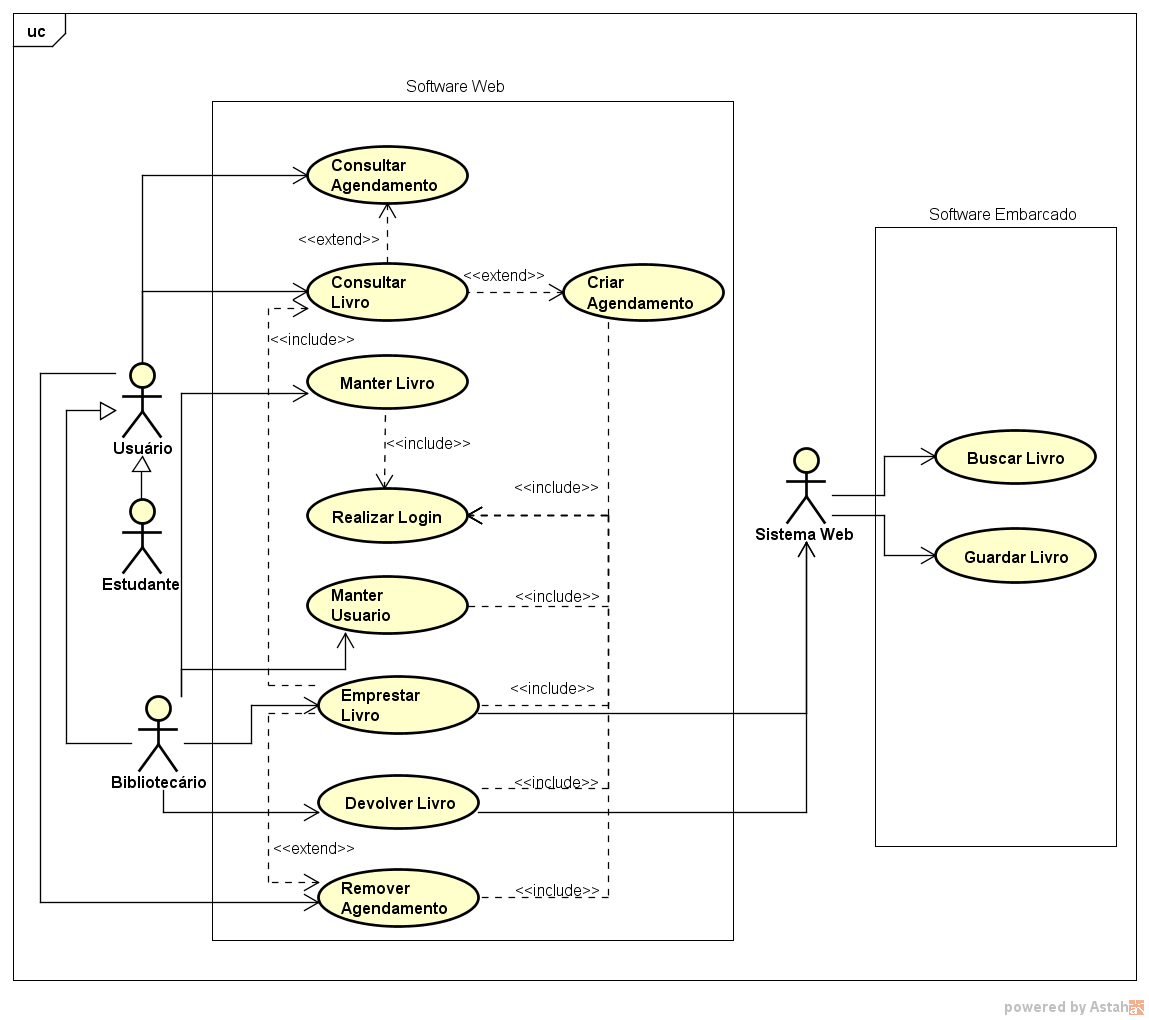
\includegraphics[scale=0.50, angle = 360]{figuras/caso_uso}
\caption[]{Diagrama de Caso de Uso para o projeto de software \textit{Bibliotech} (fonte: Autor)
}
\end{figure}
\FloatBarrier

\subsubsection{Descrição de Casos de Uso}

\begin{itemize}
\item{Consultar Agendamento}
\end{itemize}

Este caso de uso permite ao USUÁRIO consultar um agendamento realizado, e está consulta deve ser criada a partir do preenchimento de um formulário.

\begin{itemize}
\item{Consultar Livro}
\end{itemize}

Este caso de uso permite ao USUÁRIO consultar a disponibilidade de um livro no sistema, e está consulta deve ser criada a partir do preenchimento de um formulário.

\begin{itemize}
\item{Criar Agendamento}
\end{itemize}

Este caso de uso permite ao USUÁRIO criar um agendamento de solicitação de livro, e está consulta deve ser criada a partir do preenchimento de um formulário.

\begin{itemize}
\item{Manter Livro}
\end{itemize}

Este caso de uso permite ao BIBLIOTECÁRIO cadastrar, alterar, remover e consultar informações de um livro no sistema.

\begin{itemize}
\item{Realizar Login}
\end{itemize}

Este caso de uso permite ao BIBLIOTECÁRIO identificar-se para que eventuais permissões lhe sejam concedidas.

\begin{itemize}
\item{Manter Usuário}
\end{itemize}

Este caso de uso permite ao BIBLIOTECÁRIO cadastrar, alterar, remover e consultar informações de um USUÁRIO.

\begin{itemize}
\item{Emprestar Livro}
\end{itemize}

Este caso de uso permite ao BIBLIOTECÁRIO emprestar um livro a um USUÁRIO, e associar o empréstimo. Este empréstimo deve ser criado a partir do preenchimento de um formulário. 

\begin{itemize}
\item{Devolver Livro}
\end{itemize}

Este caso de uso permite ao BIBLIOTECÁRIO devolver um livro e finalizar o empréstimo realizado a um USUÁRIO. 

\begin{itemize}
\item{Remover Agendamento}
\end{itemize}

Este caso de uso permite ao BIBLIOTECÁRIO remover um agendamento de solicitação de livro,e está consulta deve ser criada a partir do preenchimento de um formulário.

\begin{itemize}
\item{Buscar Livro}
\end{itemize}

Este caso de uso permite ao SISTEMA \textit{WEB} solicitar ao robô a busca física de um livro em seu respectivo endereço físico.

\begin{itemize}
\item{Guardar Livro}
\end{itemize}

Este caso de uso permite ao SISTEMA \textit{WEB} solicitar ao robô devolução física de um livro em seu respectivo endereço físico.


\subsection[Protótipos]{Protótipos}
Para facilitar a visão de como será o produto de software, a equipe desenvolveu alguns protótipos. Os protótipos permitem que os stakeholders interajam com o produto, assim eles podem ter uma noção de o produto será, e como utilizar o produto \cite{preece2005}. 

A maioria das funcionalidades necessita que o usuário esteja logado. A imagem abaixo mostra o protótipo da tela de login: 

\begin{figure}[!h]
\centering
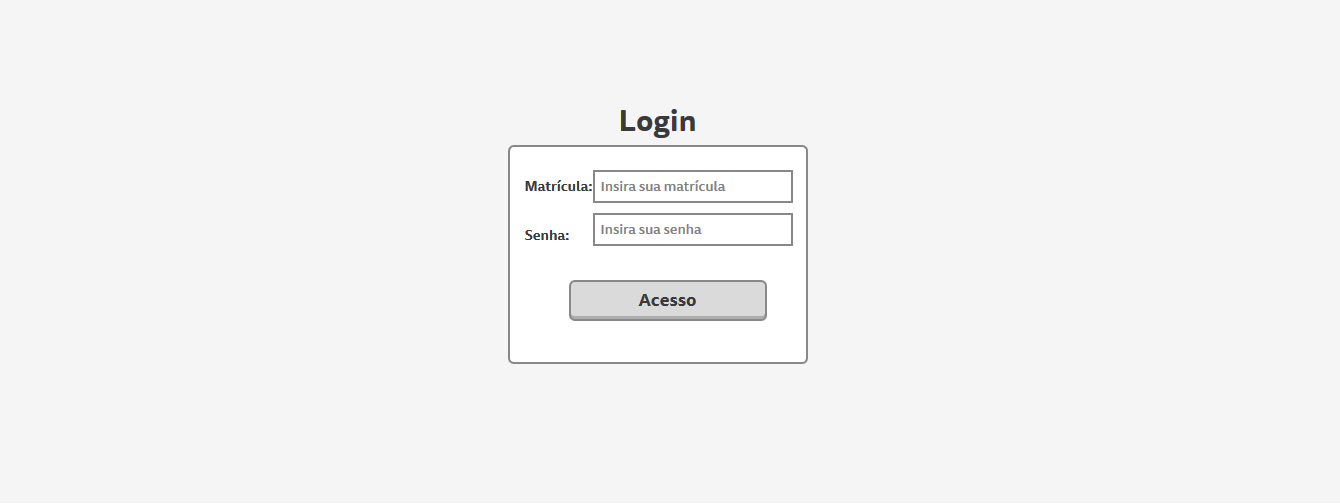
\includegraphics[scale=0.40, angle = 360]{figuras/prototipo1}
\caption[]{Tela de Login da Aplicação Web (fonte: Autor)}
\label{Tela de Login da Aplicação Web}
\end{figure}
\FloatBarrier

Após ter realizado o login, o bibliotecário consegue visualizar um menu com as opções disponíveis. A imagem abaixo apresenta esse menu:

\begin{figure}[!h]
\centering
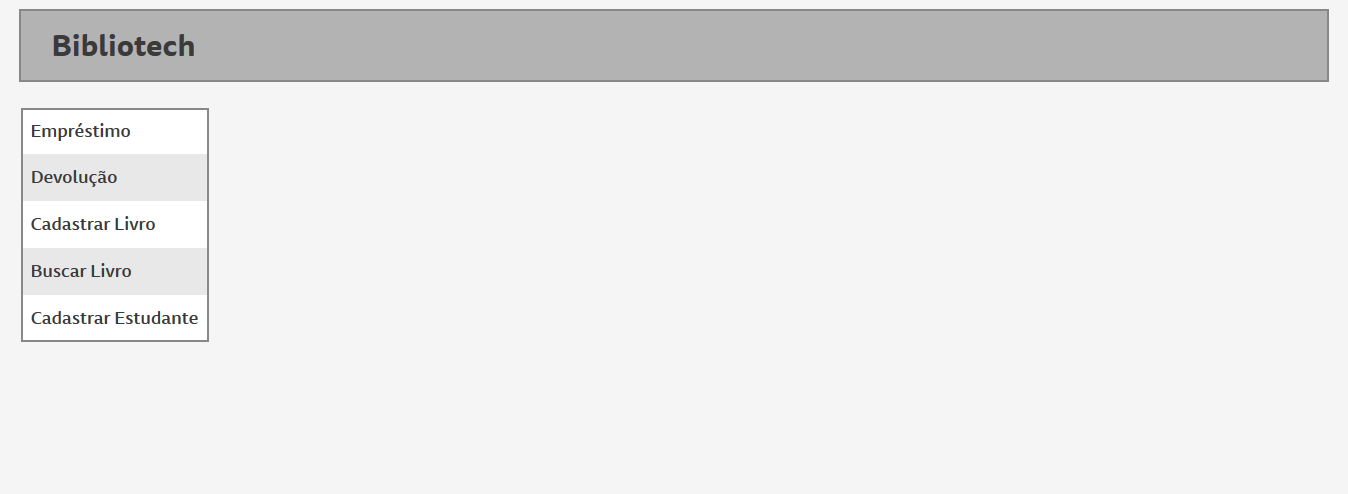
\includegraphics[scale=0.40, angle = 360]{figuras/prototipo2}
\caption[]{Tela inicial do bibliotecário (fonte: Autor)}
\label{Tela inicial do bibliotecário}
\end{figure}
\FloatBarrier

Dado o contexto de uma biblioteca, é interessante que seja realizado o cadastro de estudantes no sistema. Assim, o nosso sistema deve permitir que o bibliotecário cadastre esses alunos. A imagem abaixo mostra o protótipo do cadastro de estudantes:

\begin{figure}[!h]
\centering
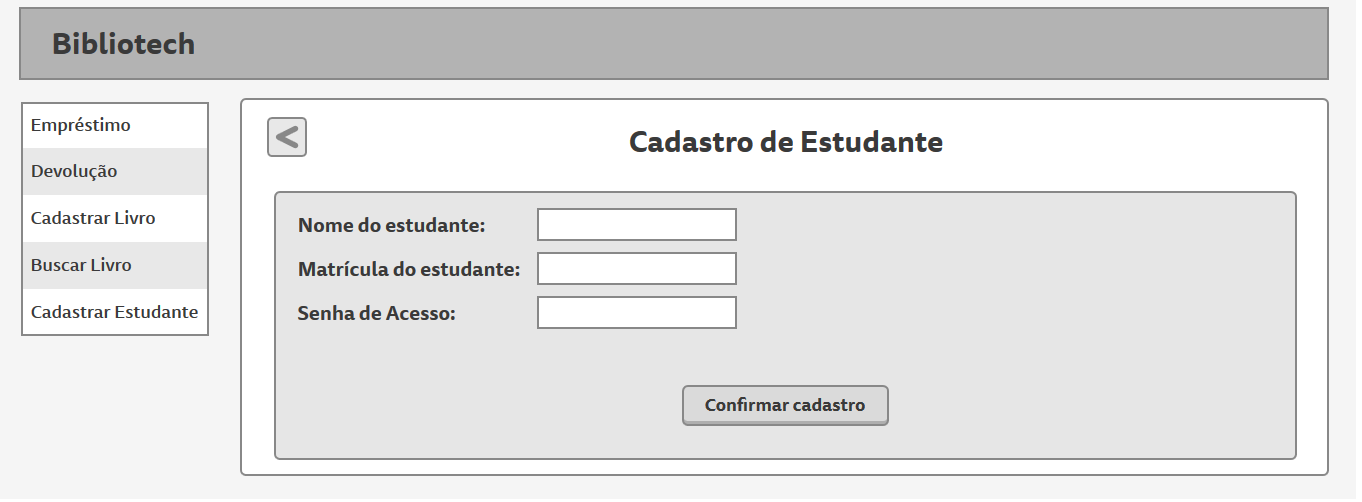
\includegraphics[scale=0.40, angle = 360]{figuras/prototipo3}
\caption[]{Tela de Cadastro de estudantes (fonte: Autor)}
\label{Tela de Cadastro de estudantes}
\end{figure}
\FloatBarrier

Também é interessante permitir ao bibliotecário o cadastro de livros e a edição de livros. No momento do cadastro, o sistema verifica uma posição disponível e aloca esse livro a uma posição. A imagem abaixo apresenta as telas do cadastro/edição de livros:

\begin{figure}[!h]
\centering
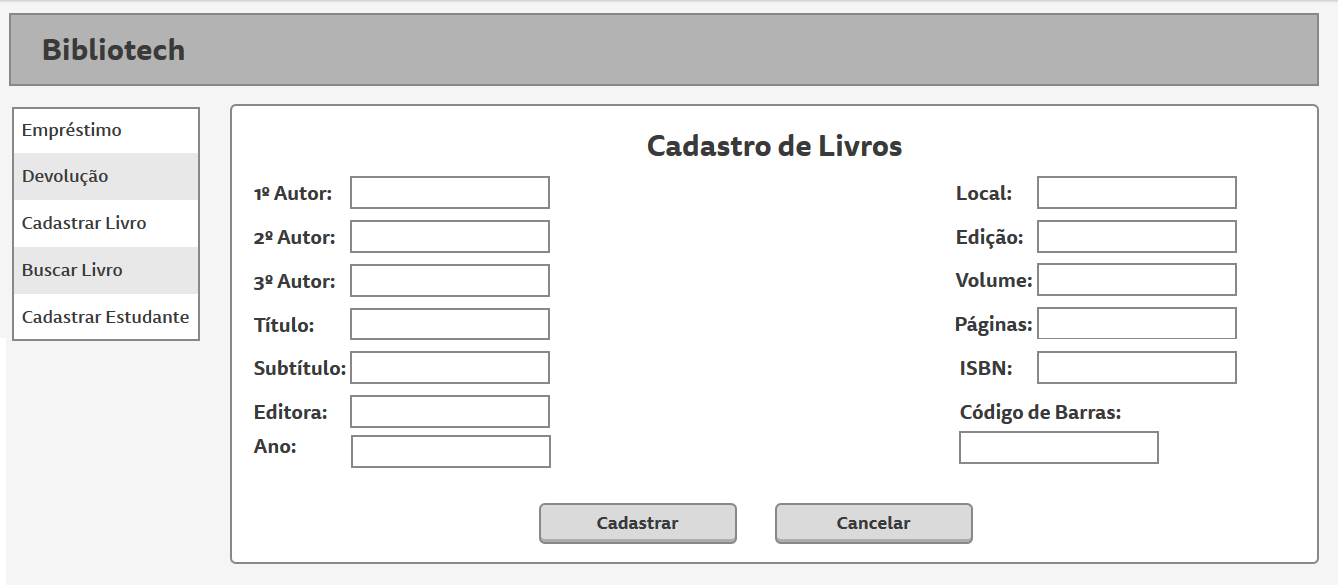
\includegraphics[scale=0.40, angle = 360]{figuras/prototipo4}
\caption[]{Tela de cadastro/edição de livros (fonte: Autor)}
\label{Tela de cadastro/edição de livros}
\end{figure}
\FloatBarrier

O sistema deverá permitir que tanto o estudante quanto o bibliotecário pesquisem livros, para realizarem eventuais consultas. A imagem abaixo mostra a tela de pesquisa:

\begin{figure}[!h]
\centering
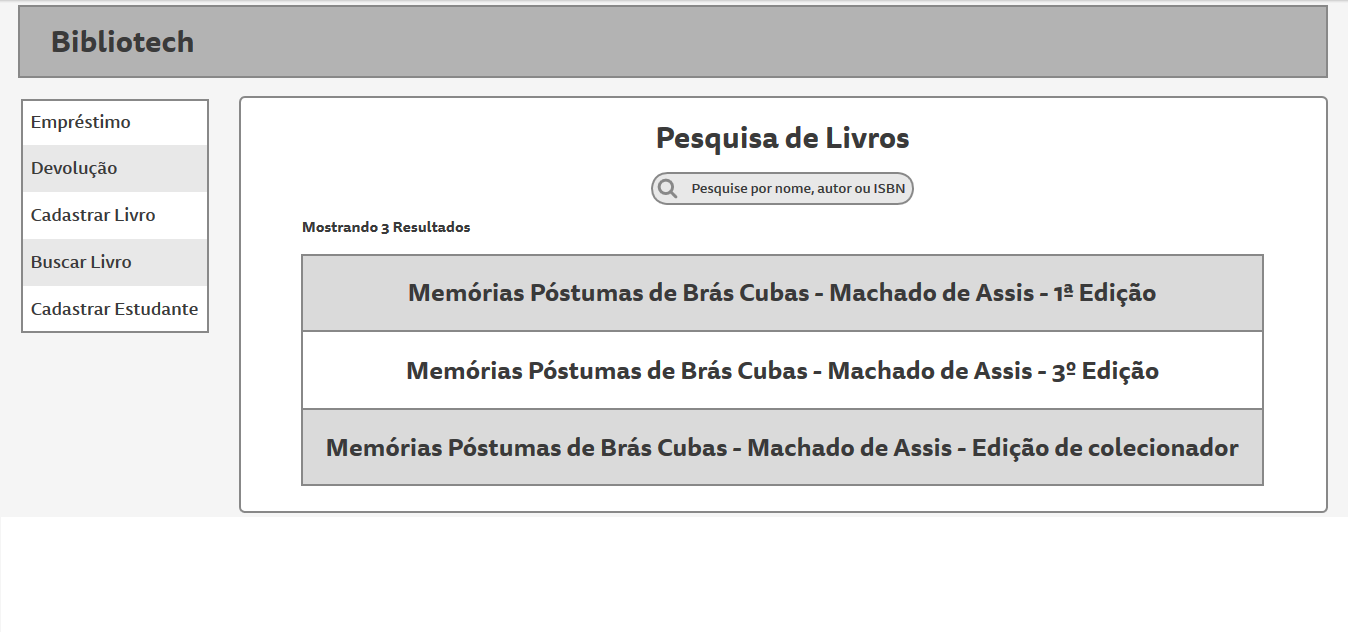
\includegraphics[scale=0.40, angle = 360]{figuras/prototipo5}
\caption[]{Tela de pesquisa de livros (fonte: Autor)}
\label{Tela de pesquisa de livros}
\end{figure}
\FloatBarrier

Após a pesquisa, o estudante ou o bibliotecário irá escolher um dos livros e realizar a consulta. Para o estudante, é informado o status do livro e uma mensagem. Caso o livro não esteja disponível, é mostrada o opção de  agendar livro. A imagem abaixo e a imagem subsequente mostra a tela de consulta do estudante e a imagem \textbf{X}, mostra a tela de agendamento:

\begin{figure}[!h]
\centering
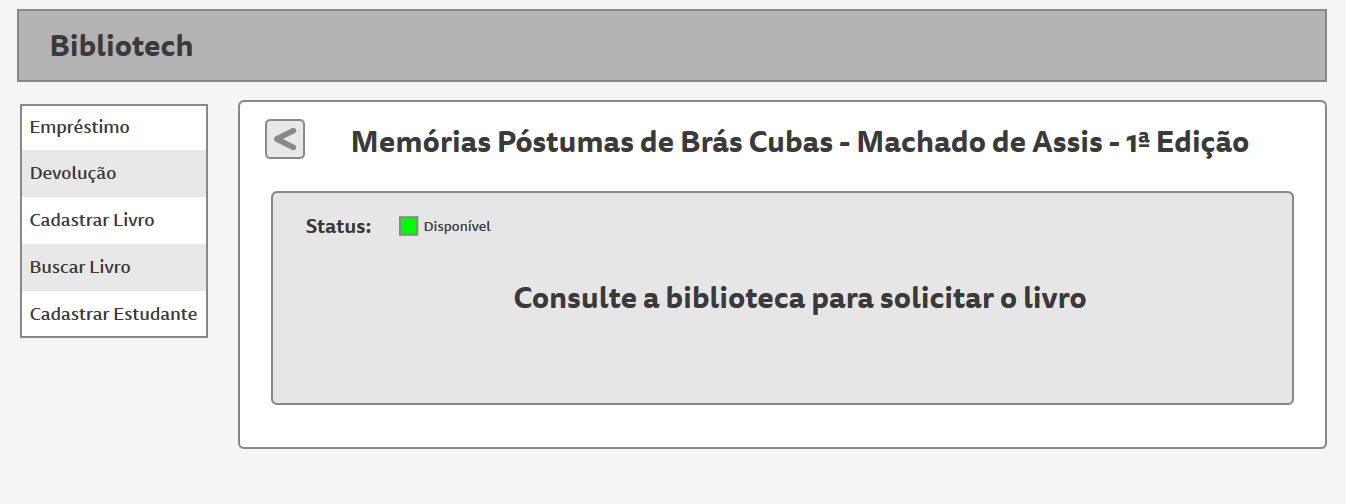
\includegraphics[scale=0.40, angle = 360]{figuras/prototipo6}
\caption[]{Tela de consulta de livro do estudante (fonte: Autor)}
\label{Tela de consulta de livro do estudante}
\end{figure}
\FloatBarrier

\begin{figure}[!h]
\centering
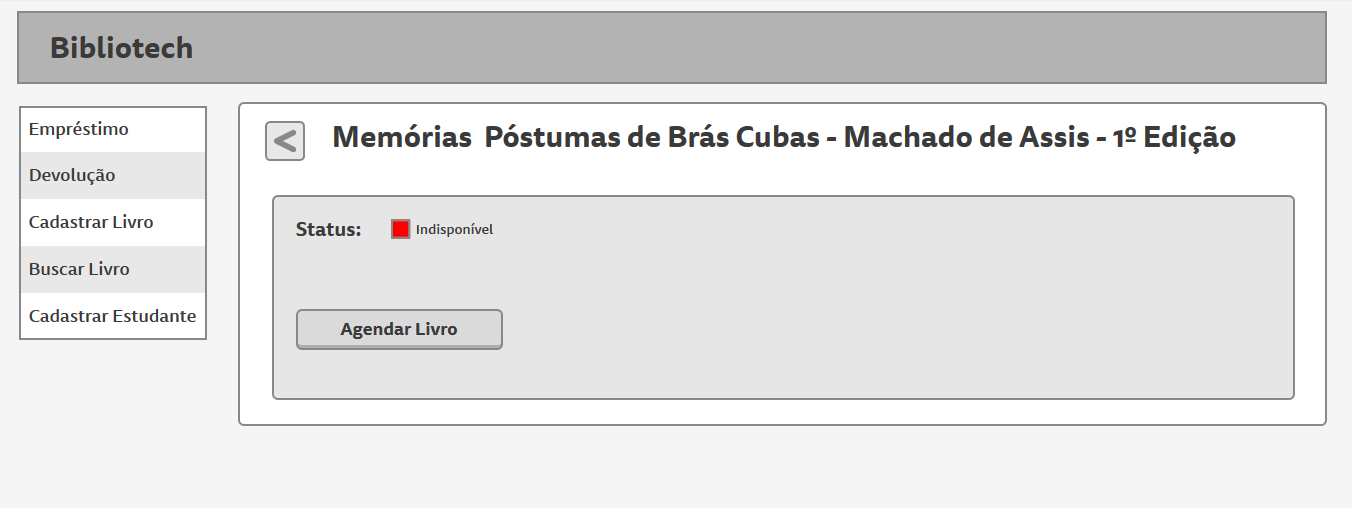
\includegraphics[scale=0.40, angle = 360]{figuras/prototipo7}
\caption[]{Tela de consulta de livro do estudante (fonte: Autor)}
\label{Tela de consulta de livro do estudante}
\end{figure}
\FloatBarrier

\begin{figure}[!h]
\centering
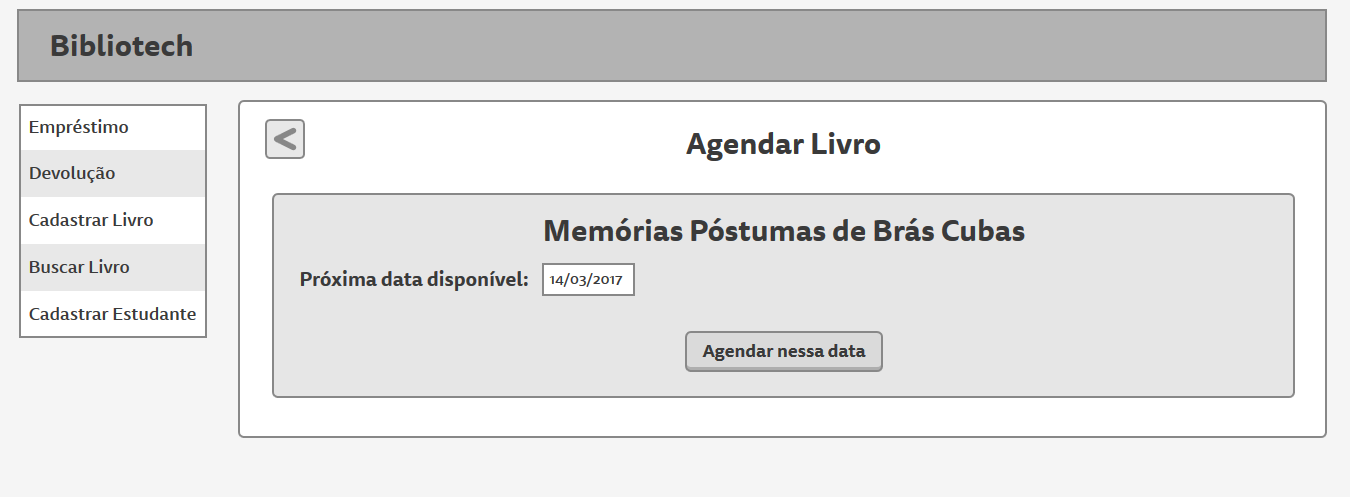
\includegraphics[scale=0.40, angle = 360]{figuras/prototipo8}
\caption[]{Tela de consulta de livro do estudante (fonte: Autor)}
\label{Tela de consulta de livro do estudante}
\end{figure}
\FloatBarrier

Na consulta, para o bibliotecário, é informado o estado do livro e um botão para iniciar o empréstimo. A imagem \textbf{X} mostra a tela de consulta do bibliotecário:

\begin{figure}[!h]
\centering
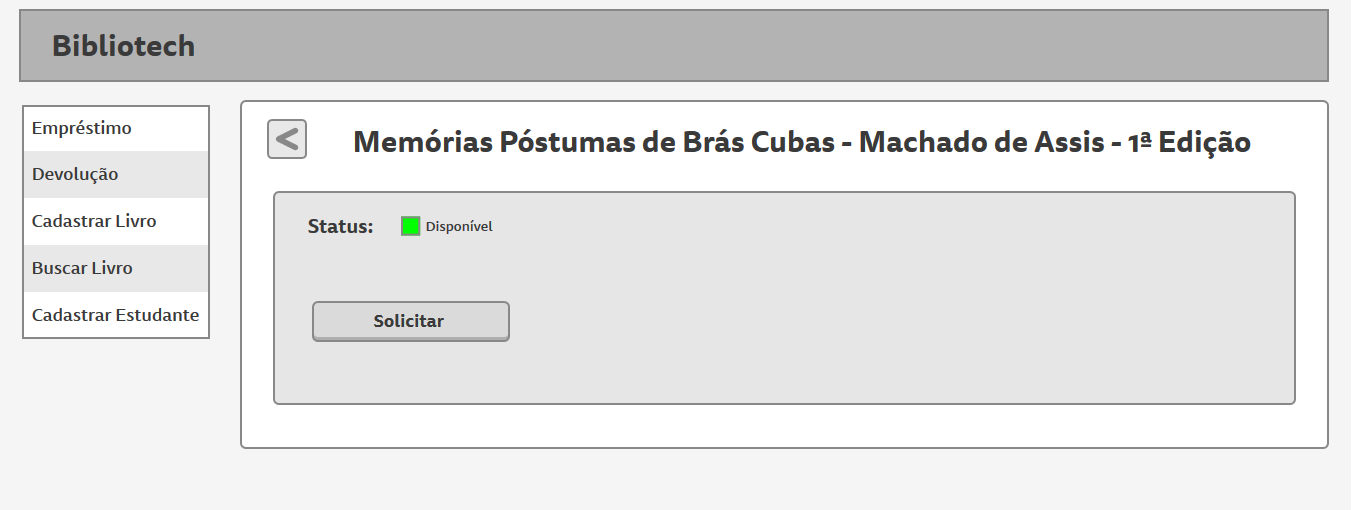
\includegraphics[scale=0.40, angle = 360]{figuras/prototipo9}
\caption[]{Tela de consulta livro bibliotecário (fonte: Autor)}
\label{Tela de consulta livro bibliotecário}
\end{figure}
\FloatBarrier

Após a solicitação do livro, o robô trará o livro para o bibliotecário e ele inserirá as informações do estudante, confirmando o empréstimo. A imagem abaixo mostra a tela de empréstimo:

\begin{figure}[!h]
\centering
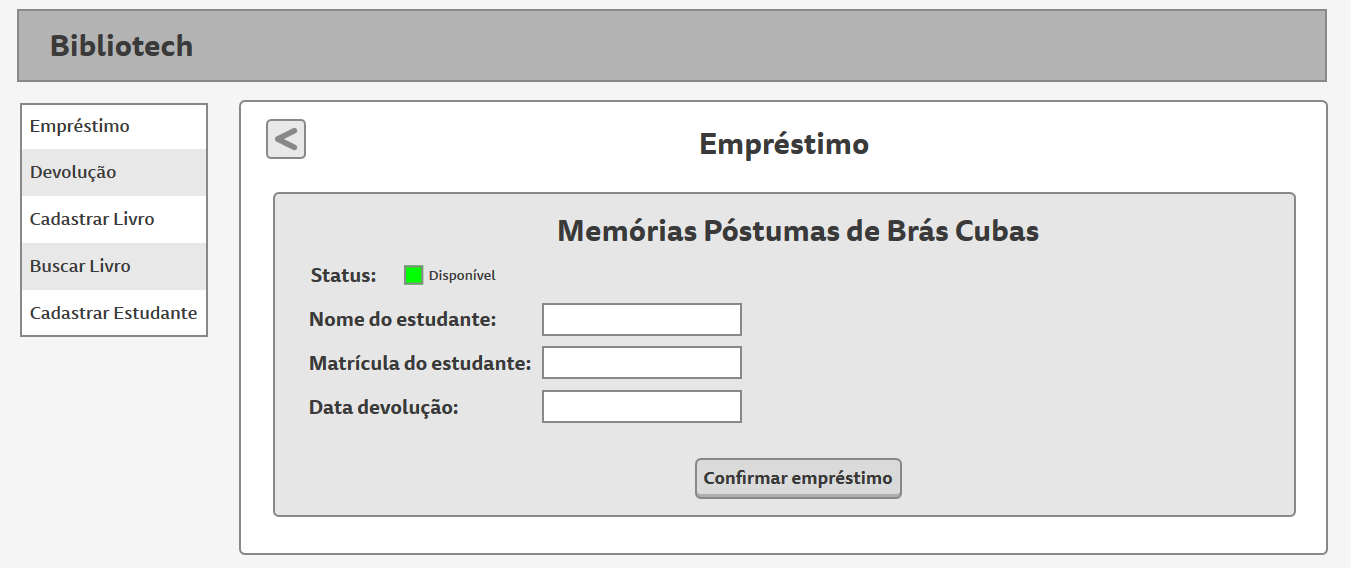
\includegraphics[scale=0.40, angle = 360]{figuras/prototipo10}
\caption[]{Tela de empréstimo de livros (fonte: Autor)}
\label{Tela de empréstimo de livros}
\end{figure}
\FloatBarrier

Quando o aluno for devolver o livro, o bibliotecário irá inserir o código de barras do livro, o sistema carregará as informações relativas ao livro, e o bibliotecário escolherá a opção de confirmar a devolução. A imagem abaixo apresenta a tela de devolução do livro:

\begin{figure}[!h]
\centering
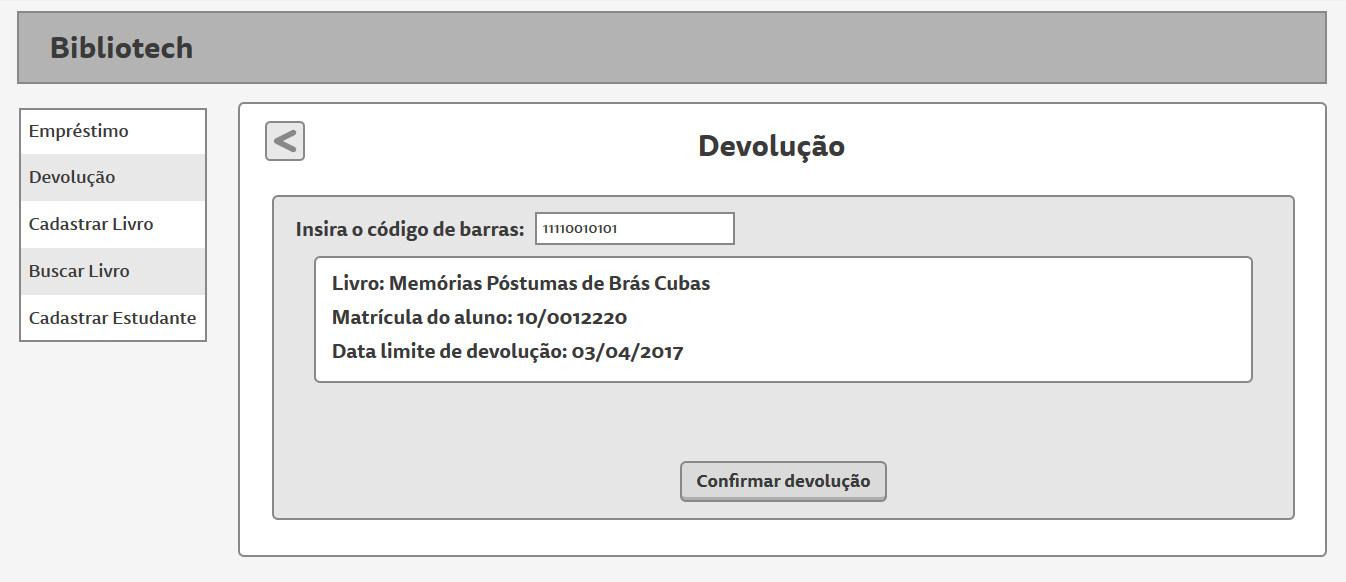
\includegraphics[scale=0.40, angle = 360]{figuras/prototipo11}
\caption[]{Tela de devolução de livros (fonte: Autor)}
\label{Tela de devolução de livros}
\end{figure}
\FloatBarrier